\chapter{Proposed Design (If any)}

The proposed platform is organised into four layers, each feeding into the next, as shown in Figure~\ref{fig:architecture}.

\begin{enumerate}
    \item \textbf{Layer 1 -- Data Ingestion:} raw transaction streams, KYC profiles, behavioural logs (login, geolocation, device), and external watchlists are ingested in real time.
    \item \textbf{Layer 2 -- Intelligence Engine:} ingested data is unified into a knowledge graph capturing entities (accounts, devices, phone numbers) and their relationships, alongside a Retrieval-Augmented Generation (RAG) and LLM core used for regulatory-document retrieval and narrative generation.
    \item \textbf{Layer 3 -- AI Agent Layer:} a set of specialised components operate on top of the shared knowledge graph and intelligence engine -- a Fraud Detection Engine (GNN and/or anomaly-detection driven), an AML Intelligence Agent for cross-account network analysis, a Transaction Risk Scoring component, a Compliance Assistant for automated SAR drafting, a Customer Risk Profiler, and a Fraud Investigation Graph for analyst-facing visualisation. Of these, the Fraud Detection/Risk Scoring component and the Compliance Assistant correspond directly to Objectives 2 and 3; the remaining components are discussed as extensions in Section~5.3.
    \item \textbf{Layer 4 -- Actions and Outputs:} the analyst dashboard, automatic transaction blocking/freezing, regulatory filing, and case-management workflow that surface the platform's outputs to a human analyst.
\end{enumerate}

A feedback loop connects analyst decisions (confirmed fraud, cleared false positives) back into Layer 1, so that the underlying models are continuously retrained on real outcomes rather than remaining static after initial training.

\begin{figure}[htbp]
    \centering
    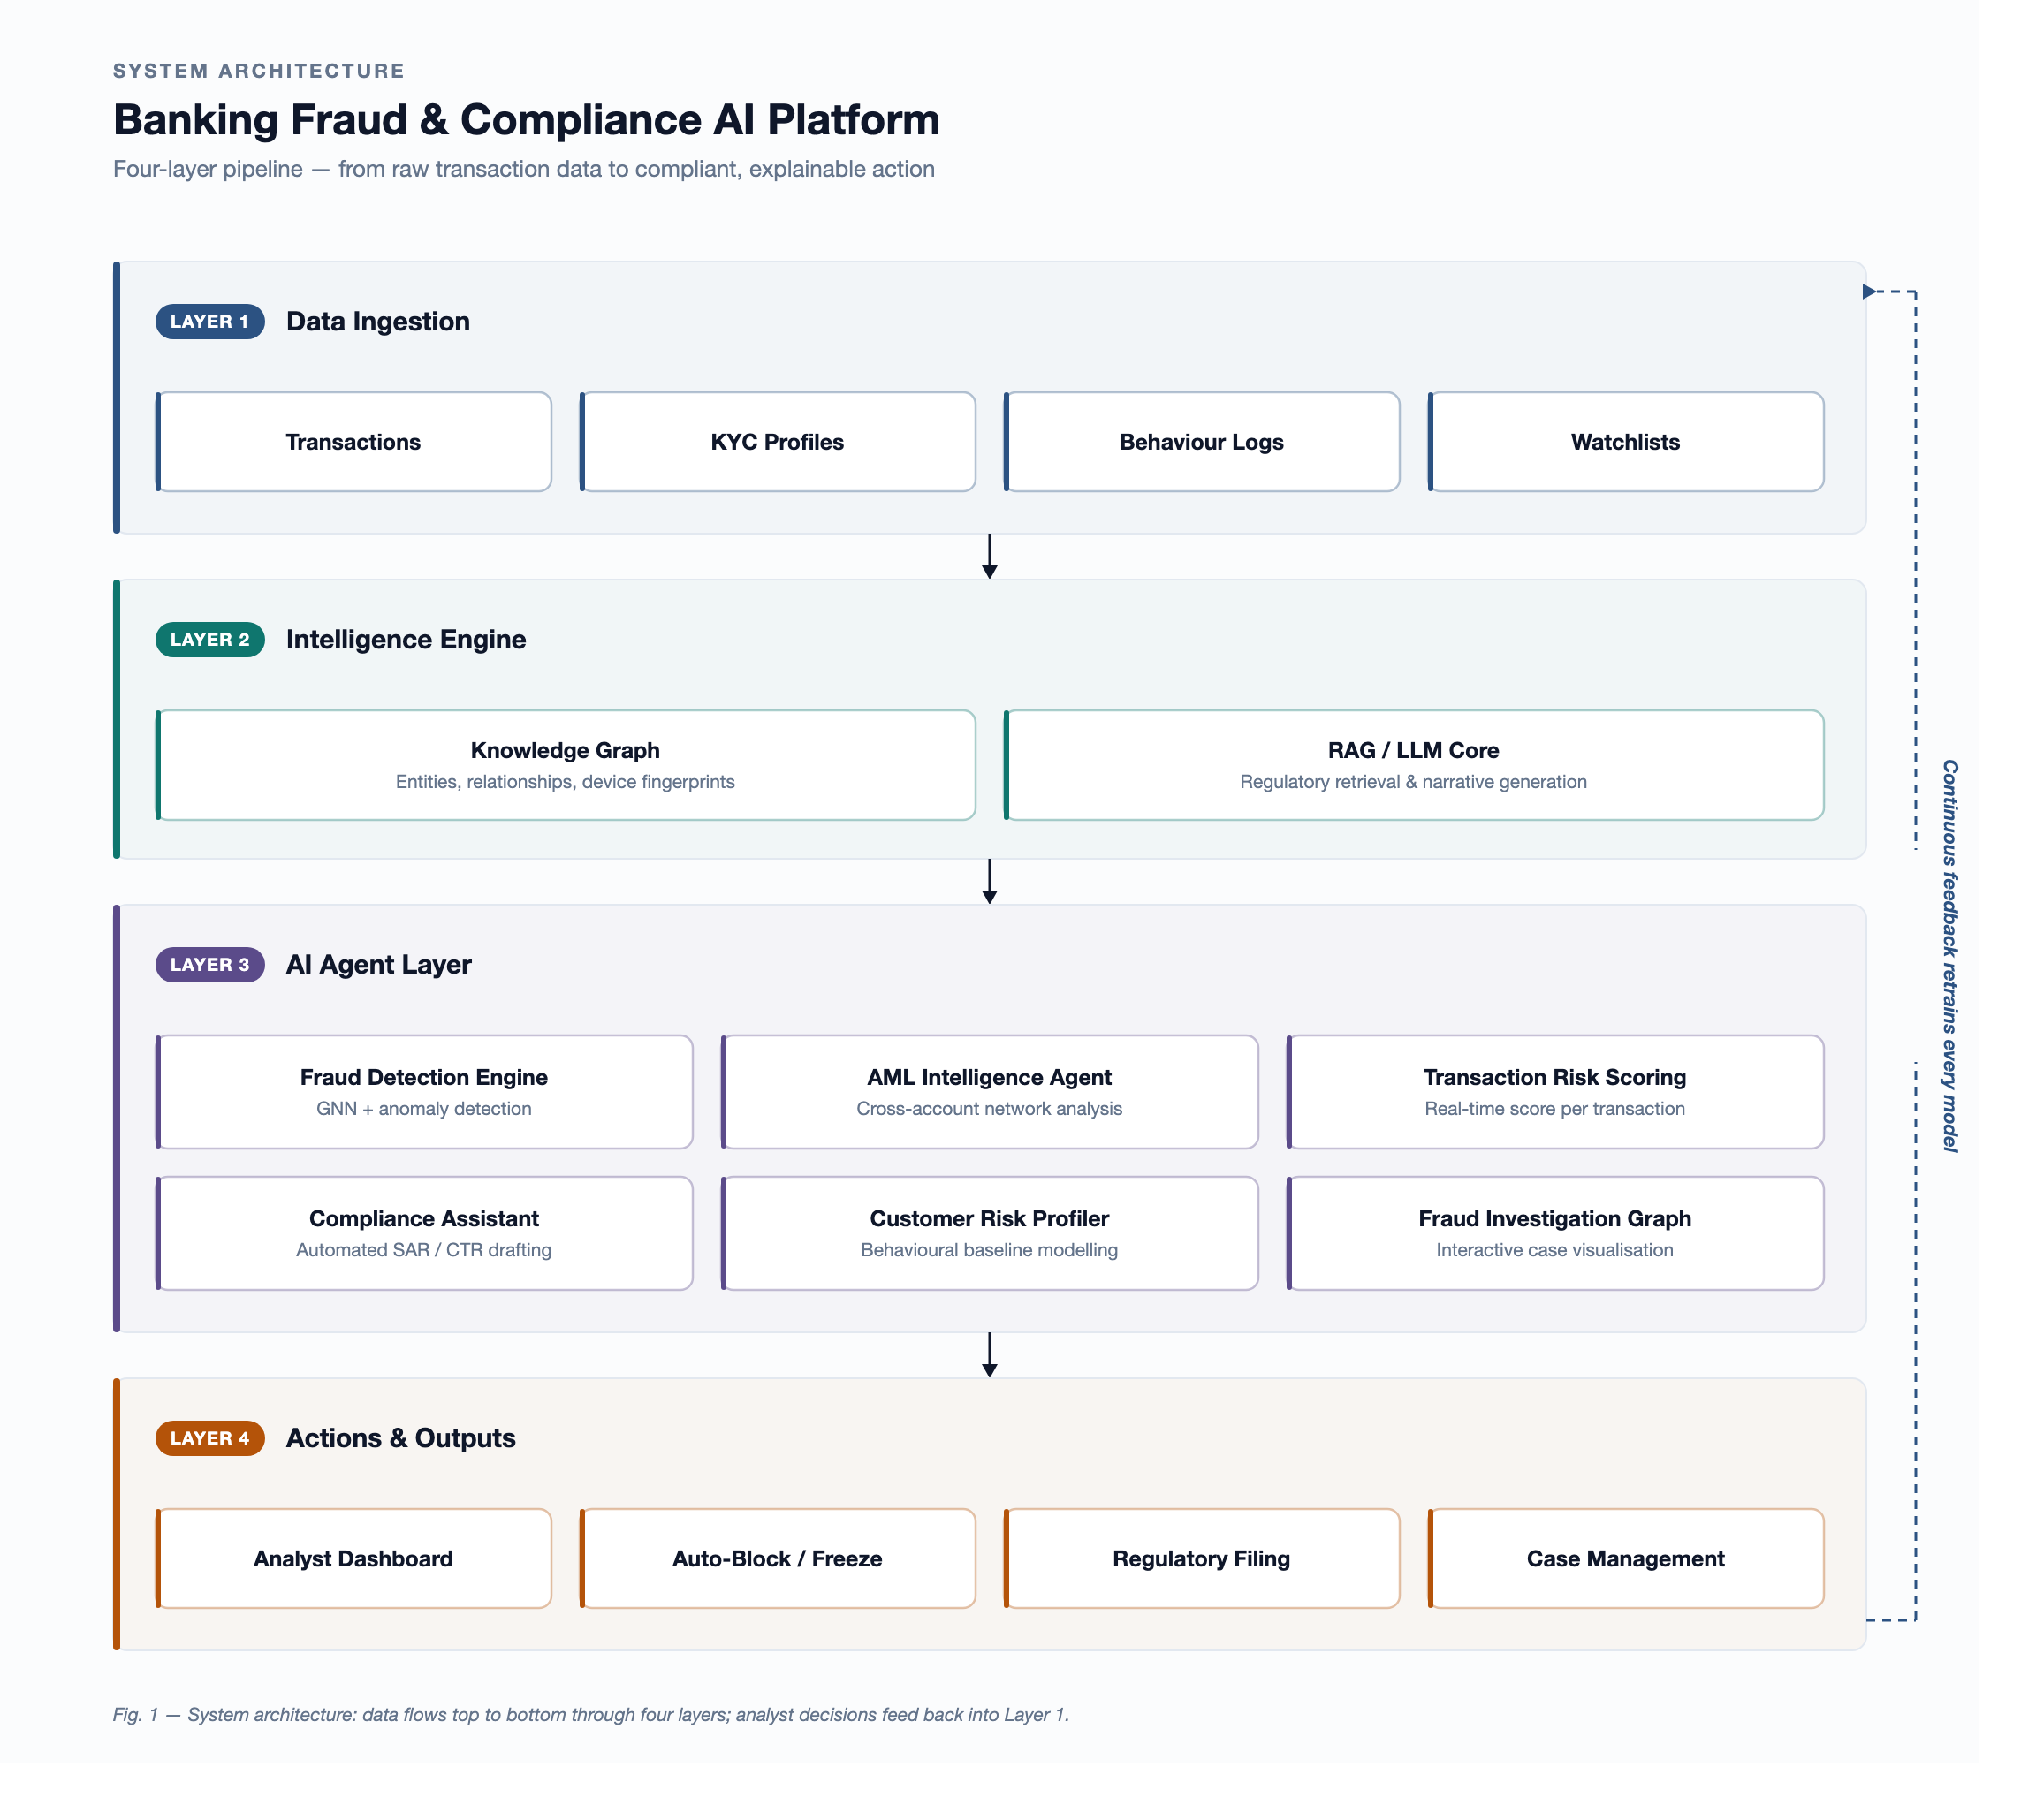
\includegraphics[width=0.95\textwidth]{system_architecture.png}
    \caption{Four-layer system architecture of the proposed platform}
    \label{fig:architecture}
\end{figure}

\section{End-to-End Flow}

Figure~\ref{fig:flow} traces a representative scenario -- a money-mule account being used to move funds overseas -- through all four layers of the platform, from the initial transaction through to a closed, compliant case.

\begin{enumerate}
    \item \textbf{Transaction initiated:} an overseas wire transfer is streamed in real time into the intelligence engine.
    \item \textbf{Risk score computed:} the Transaction Risk Scoring component evaluates the transaction against the account's behavioural baseline (device novelty, time-of-day deviation, amount deviation), producing a preliminary risk score.
    \item \textbf{Knowledge graph queried:} the knowledge graph is queried for the account's connections, revealing that its registered phone number and device fingerprint are shared with several other recently opened accounts -- raising the risk score substantially.
    \item \textbf{AML network analysis:} the AML Intelligence Agent maps the full network of connected accounts and recognises a known layering/structuring pattern, where funds are moved through several accounts in amounts just below regulatory reporting thresholds.
    \item \textbf{Transaction auto-frozen:} the transaction is automatically blocked before completion, and the case is pushed to the analyst dashboard with a pre-built investigation summary.
    \item \textbf{SAR auto-generated:} the Compliance Assistant retrieves the relevant regulatory text via RAG and drafts a complete SAR narrative, citing the specific transactions and regulatory clauses that justify the filing.
    \item \textbf{Analyst review and feedback:} the analyst reviews the visualised network and the generated SAR, confirms the case, and this outcome is logged to retrain the underlying models for future cases.
\end{enumerate}

\begin{figure}[htbp]
    \centering
    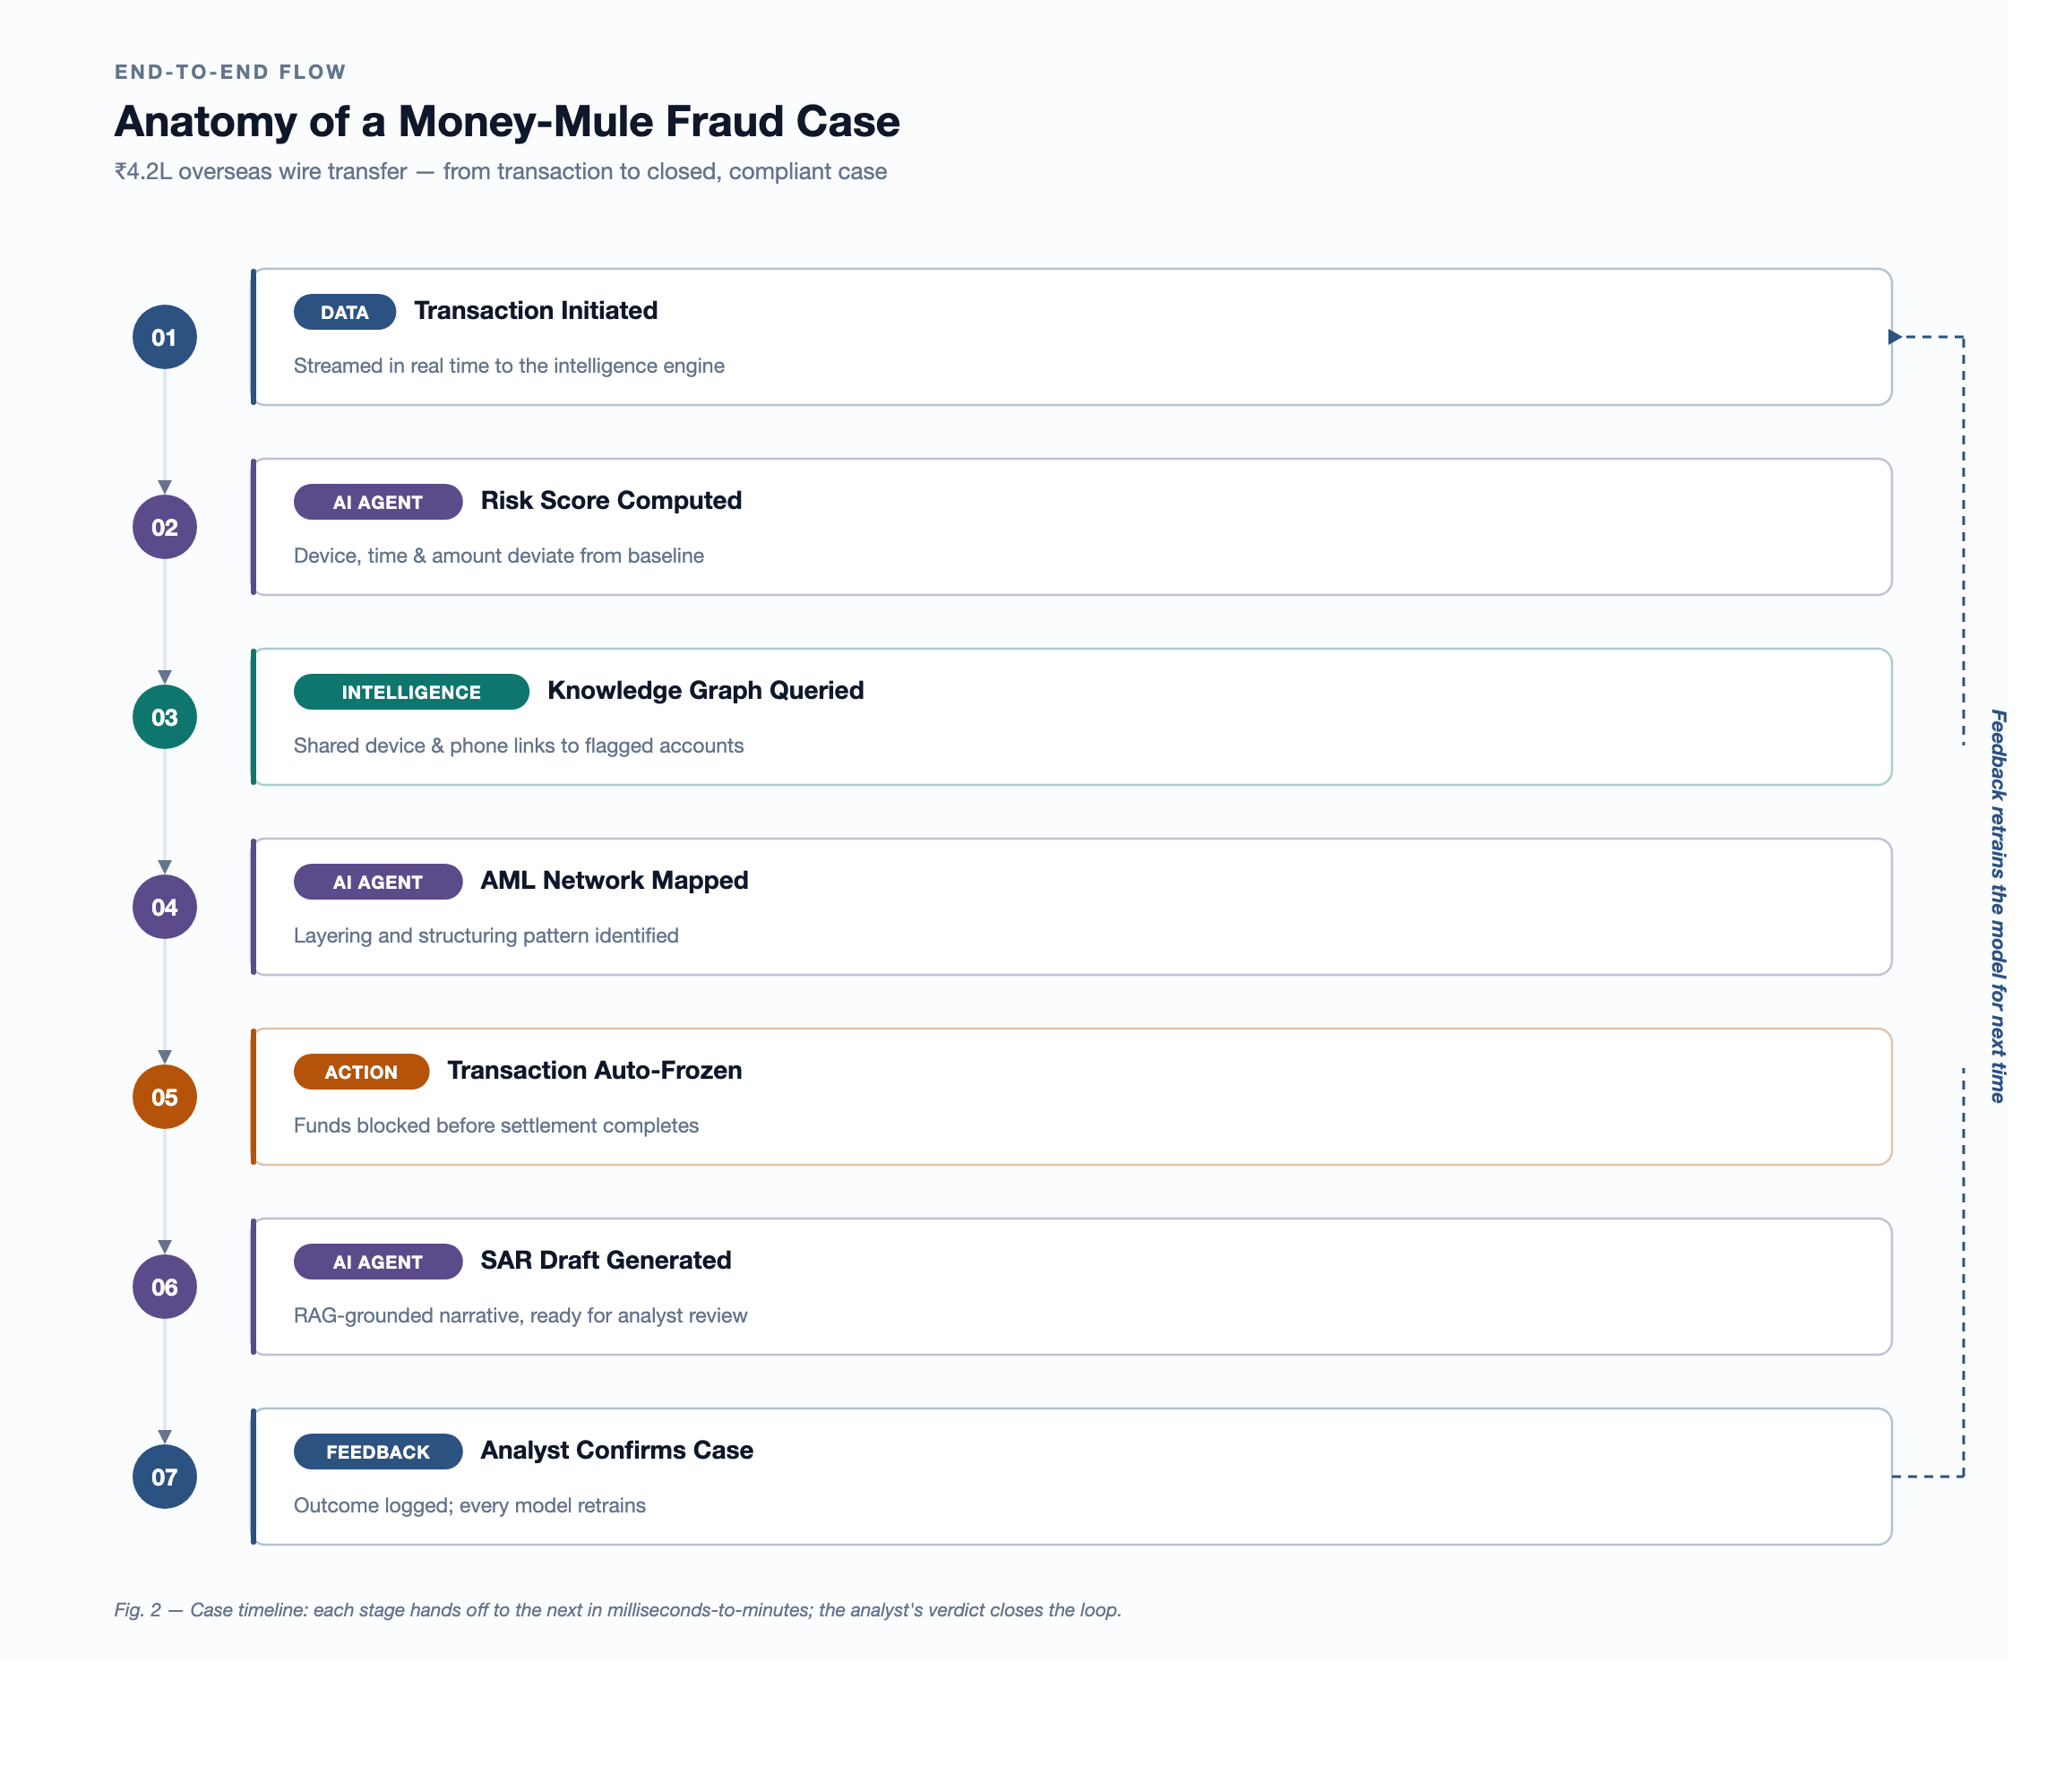
\includegraphics[width=0.95\textwidth]{end_to_end_flow.png}
    \caption{End-to-end flow for a representative money-mule fraud case}
    \label{fig:flow}
\end{figure}

\section{Scope for the Present Mini-Project}

Given the timeline available for this mini-project, implementation effort is prioritised on the three components that map directly to the objectives stated in Chapter~4: the knowledge graph (Layer 2), the transaction risk-scoring model (part of Layer 3), and the RAG-based Compliance Assistant (part of Layer 3). The remaining Layer 3 components -- the dedicated AML network agent, the continuously updated customer risk profiler, and the interactive fraud-investigation graph UI -- along with full production-grade deployment (Layer 4 automation, containerised infrastructure), are treated as extensions beyond the current scope and are discussed as future work in Chapter~6.
